\section{Chọn dầu bôi trơn cho hộp giảm tốc}
Ta có công thức:
\[
    X_{br} = \frac{10^{-5}H_{HV}\sigma_H^2}{v} = \frac{10^{-5}.260.314,887^2}{1,38} = 186,812
\]
Trong đó: 
\begin{itemize}
    \item $v = 1,38 m/s$
    \item $H_{HV} = 260MPa$
    \item   $\sigma_H = 314,887MPa$
\end{itemize}
Theo đồ thị hình 13.9a/505, ta chọn dầu bôi trơn có $v_{50} = 73 cSt$. Khi đó độ nhớt ở nhiệt độ $40^oC$ là $v_{40} = v_{50}(\frac{40}{50})^3 = 37,376 cSt$.
\begin{figure}[H]
    \centering
    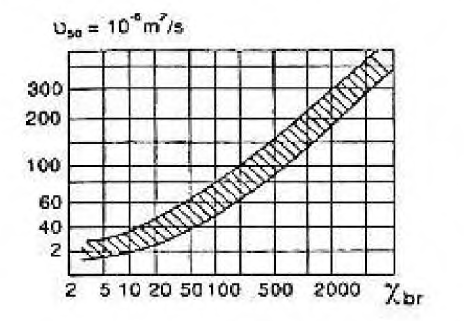
\includegraphics[width=0.4\textwidth]{pictures/nhot1.png}
    \caption{Sự phụ thuộc độ nhớt v theo x của bánh răng}
\end{figure}
Do đó theo bảng 13.1 ta chọn dầu bôi trơn ISO VG 46.
\begin{figure}[H]
    \centering
    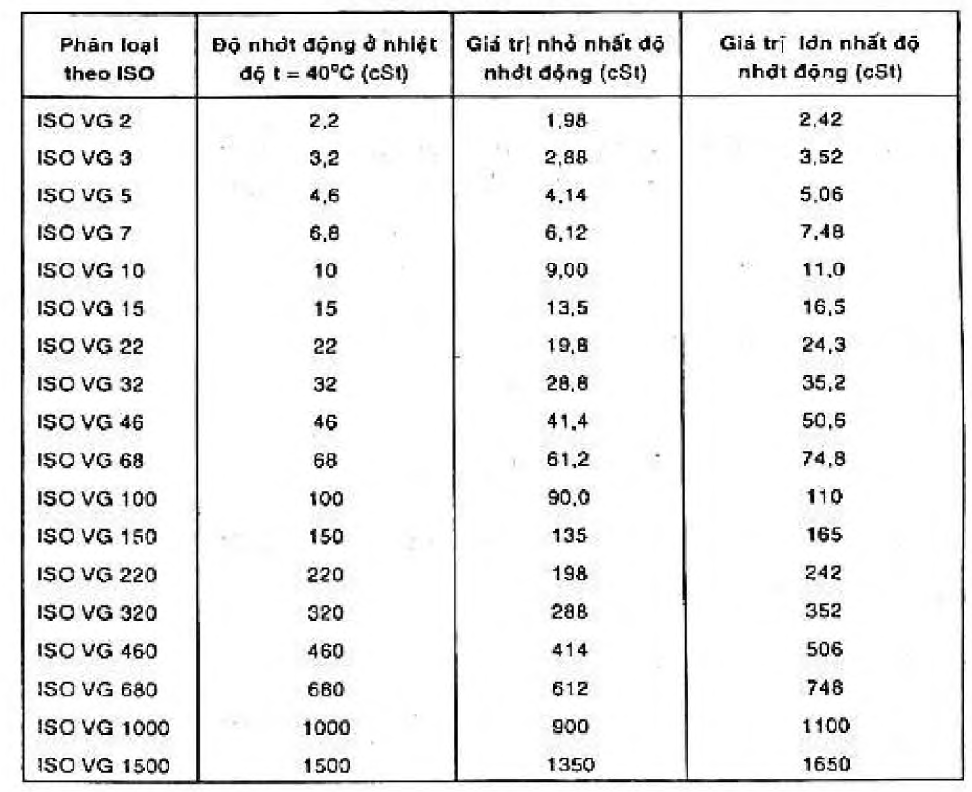
\includegraphics[width=0.5\textwidth]{pictures/nhot2.png}
    \caption{Dầu bôi trơn ISO VG}
\end{figure}
\cleardoublepage